\tikzstyle{simpleNode}=[circle,draw,thick,minimum width=0.8cm] 

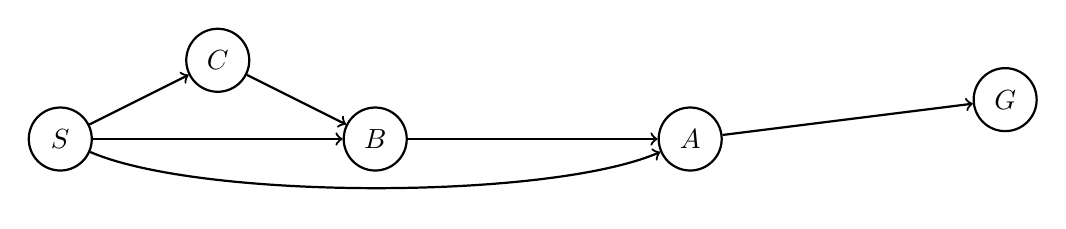
\begin{tikzpicture}[xscale=4,->=stealth]

  \node[simpleNode] (s) at (0,0) {$S$};
  \node[simpleNode] (b) at (1,0) {$B$};
  \node[simpleNode] (a) at (2,0) {$A$};
  \node[simpleNode] (g) at (3,0.5) {$G$};
  \node[simpleNode] (c) at (0.5,1) {$C$};

  \path[->,draw,thick](s)--(b);
  \path[->,draw,thick](b)--(a);
  \path[->,draw,thick](a)--(g);
  \path[->,draw,thick](s)--(c);
  \path[->,draw,thick](c)--(b);
  \path[->,draw,thick](s) to[bend right=60](a);

\end{tikzpicture}
